\chapter{DHCPv4}

\section{Operation}

DHCPv4 works in a client/server mode. When a client communicates with a DHCPv4 server, the server assigns or leases an IPv4 address to that client. The client connects to the network with that leased IP address until the lease expires.\\

The client must contact the DHCP server periodically to extend the lease. This lease mechanism ensures that clients that move or power off do not keep addresses that they no longer need. When a lease expires, the DHCP server returns the address to the pool where it can be reallocated as necessary.\\

\subsection{Lease origination}

When the client boots (or otherwise wants to join a network), it begins DORA\footnote{DORA = Discovery, Offer, Request, Acknowledgement} process to obtain a lease.

\begin{enumerate}
\item A client starts the process with a broadcast \textbf{DHCP-DISCOVER} message to finds available DHCPv4 servers.

\item When the DHCPv4 server receives a DHCP-DISCOVER message, it reserves an available IPv4 address to lease to the client. It then sends a \textbf{DHCP-OFFER} message to the requesting client. The server also creates an ARP entry consisting of the MAC address of the requesting client and the leased IPv4 address of the client.

\item When the client receives the DHCP-OFFER from the server, it broadcasts\textbf{DHCP-REQUEST} messages. The DHCP-REQUEST serves as an acceptance notice to the selected server and an implicit decline to any other servers.

\item On receiving the DHCP-REQUEST message, the server verifies the lease information with an ICMP ping to that address to ensure it is not being used already. If there is \emph{no} ICMP echo reply, then the address is is not being used by any client. Otherwise, that address is being used and the server has to send DHCP-OFFER again.

\item DHCP server sends  unicast DHCP-ACK message to the client. The DHCP-ACK message informs the client that the IP address is valid. Because The DHCP-ACK message is a duplicate of the DHCP-OFFER, it also provides IP information for the client.

\item When the client receives the DHCPACK message, performs an ARP lookup for the assigned address.
If there is no reply to the ARP, the client knows that the IPv4 address is valid and starts using it as its own.
\end{enumerate}



\subsection{Lease renewal}

\begin{enumerate}
\item Before the lease expires, the client sends a DHCPREQUEST message directly to DHCPv4 server. If a DHCPACK is not received within a specified amount of time, the client broadcasts another DHCPREQUEST so that one of the other DHCPv4 servers can extend the lease.

\item On receiving the DHCPREQUEST message, the server verifies the lease information by returning a DHCPACK
\end{enumerate}

\subsection{Relay agent}

Sometimes, network clients are not on the same subnet as DHCP servers. Because routers do not forward broadcasts, the DHCP-REQUEST from clients are not sent to DHCP server.\\

Cisco offers a solution called Cisco IOS helper address. This solution enables a router to forward DHCP-REQUEST broadcasts to the DHCPv4 server. When
a router forwards address assignment/parameter requests, it is acting as a DHCPv4 \emph{relay agent}.

\section{Message}

DHCPv4 messages UDP encapsulation. The server uses port 67, the client uses port 68.

\subsection{Message format}

\paragraph{Operation (OP) code}specifies general type of message: request (1), reply (2).

\begin{figure}[hbtp]
\caption{DHCPv4 message format}
\centering
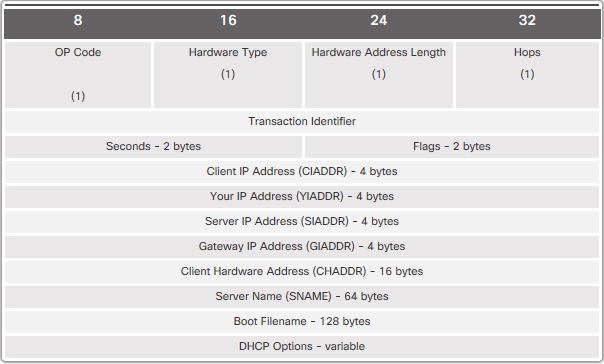
\includegraphics[ width=0.8\textwidth ]{pictures/DHCPmessage.PNG}
\end{figure}

\paragraph{Hardware type} Ethernet (1), Frame Relay (15), Serial (20)

\paragraph{Hop}Controls the forwarding of messages. Set to 0 by a client before transmitting a request.

\paragraph{Transaction identifier} used by client to match the request with replies from DHCPv4 server.

\paragraph{Seconds} amount of time (in seconds) elapsed since a client attempted to acquire or renew a lease.

\paragraph{Flag}Used by a client that does not know its IPv4 address when it sends a
request. Only one of the 16 bits—the broadcast flag—is used. A value of 1 in
this field tells the DHCPv4 server or relay agent receiving the request that the
reply should be sent as a broadcast.

\subsection{DHCP-DISCOVER}

When the client boots, it has no way of knowing the subnet to which it belongs. Therefore, destination
IPv4 address of DCHP-DISCOVER is 255.255.255.255, the destination MAC address is FF:FF:FF:FF:FF:FF. The source MAC address is the MAC address of the client. The client does not have a configured IPv4 address
yet, so the source IPv4 address is 0.0.0.0 

\subsection{DHCP-OFFER}

DHCP-OFFER contains initial configuration information
for the client: IPv4 address for client, subnet mask, lease duration, and IPv4 address of the DHCPv4 server. The DHCPOFFER message can be configured to include other information, such as the lease renewal time and DNS address.


\section{Configuration}

\subsection{DHCPv4 server}

\begin{description}
\item[Step 1. Exclude addresses]Some IPv4 addresses in a pool are assigned to network devices that require static address assignments. Therefore, these IPv4 addresses should not be assigned to other devices.

\begin{verbatim}
R1(config)# ip dhcp excluded-address <ip-address>
R1(config)# ip dhcp excluded-address 192.168.10.1

R1(config)# ip dhcp excluded-address <range-of-address>
R1(config)# ip dhcp excluded-address 192.168.10.1 192.168.10.9
\end{verbatim}

\item[Step 2. Configure address pool]Define a pool of addresses to assign to clients.

\begin{verbatim}
R1(config)# ip dhcp pool <pool-name>
R1(dhcp-config)# network <network-range>

R1(config)# ip dhcp pool LAN-POOL-1
R1(dhcp-config)# network 192.168.10.0 255.255.255.0
\end{verbatim}

\item[Step 3. Default gateway]Define the default gateway router for clients. 

\begin{verbatim}
R1(dhcp-config)# default-router 192.168.10.1
\end{verbatim}

\item[Step 4. Relay agent]If network clients are not on the same subnet as DHCP servers, configure the default gateway as a relay agent.

\begin{verbatim}
R1(config)# interface g0/0
R1(config-if)# ip helper-address 192.168.11.6
\end{verbatim}

\item[Step 4 (Optional). Other DHCP specifics]\\

\begin{verbatim}
R1(dhcp-config)# dns-server 192.168.11.5
R1(dhcp-config)# domain-name example.com
\end{verbatim}

\item[Step 5. Verification] The \verb|show ip dhcp binding| command displays a list of all IPv4 address to MACaddress bindings that have been provided by the DHCPv4 service. The \verb|show ip dhcp server statistics| command verifies that messages are being received or sent by the router. This command displays count information regarding the number of DHCPv4 messages that have been sent and received.

\begin{verbatim}
R1# show run | sec dhcp
R1# show ip dhcp binding
R1# show ip dhcp statistics
\end{verbatim}
\end{description}

\subsection{DHCPv4 client}

\begin{verbatim}
SOHO(config)# interface g0/1
SOHO(config-if)# ip address dhc
SOHO(config-if)# no shutdown
\end{verbatim}


\chapter{DHCPv6}

\section{Operation}

\subsection{SLAAC}

Stateless Address AutoConfiguration (SLAAC) is enabled by default. Both the M flag and the O flag are set to 0 in the RA. In SLAAC, a host automatically obtains its IP configuration from an IPv6-enabled router. The host generates its own unique IPv6 address. A DHCPv6 server is not required. SLAAC operation includes the following steps:

\begin{enumerate}
\item Client asks for IPv6 configuration by sending an RS to the router R1.
\item R1 receives the RS message and responds with an RA message.
\item PC1 receives the RA, and uses the information in the message to create its own IPv6 global unicast address. 
\item Because SLAAC is a stateless process, PC1 must verify that this newly created IPv6 address is unique using DAD process.
\end{enumerate}

\subsection{SLAAC and Stateless DHCPv6}

A host obtains IP configuration (prefix, prefix-length, default gateway) using SLAAC and additional information (DNS server, domain name, etc.) from a stateless DHCPv6 server. The host generates its own unique IPv6 address. 

\subsection{Stateful DHCPv6}

In stateful DHCPv6, the RA message informs the client not to use the information in the RA message. All addressing information and configuration information must be obtained from a stateful DHCPv6 server. This is known as \emph{stateful} DHCPv6 because the DHCPv6 server maintains IPv6 state information.\\

DHCPv6 messages from the server to the client use UDP destination port 546. The client sends DHCPv6 messages to the server using UDP destination port 547.

\section{Message}

\begin{itemize}
\item \textbf{Router solicitation (RS):} The client sends an RS message to the router. The destination address of the message is \textbf{all-routers} multicast address \textbf{FF02::2}.

\item \textbf{Router advertisement (RA):} RAs are sent by routers to provide IP configuration to clients. The RA message includes IPv6 configuration for clients (prefix, prefix-length, DNS server, MTU, and default gateway information). A router sends an RA message periodically (every 200s) or in response to an RS message. RA messages are always sent to the IPv6 \textbf{all-nodes} multicast address \textbf{FF02::1}.
\end{itemize}

The two flags are the Managed Address Configuration flag (M flag) and the
Other Configuration flag (O flag).
Using different combinations of the M and O flags, RA messages have one of three
addressing options for the IPv6 device, as shown in Figure 8-13:
■ SLAAC (Router Advertisement only)
■ Stateless DHCPv6 (Router Advertisement and DHCPv6)
■ Stateful DHCPv6 (DHCPv6 only)


\subsection{Client IPv6}

The
IPv6 global unicast address is created by combining the prefix from RA and an
Interface ID using either EUI-64 or a randomly generated value.

PC1 now has a 64-bit network prefix but needs a 64-bit interface ID
(IID) to create a global unicast address.
PC1 can create its own unique IID in two ways:
● EUI-64—Using the EUI-64 process, PC1 creates an IID using its 48-bit MAC
address.
● Randomly generated—The 64-bit IID can be a random number that the client
operating system generates.
PC1 can create a 128-bit IPv6 global unicast address by combining the 64-bit
prefix with the 64-bit ID. PC1 uses the link-local address of the router as its IPv6

\subsection{DAD process}

PC1 sends an ICMPv6 neighbor
solicitation (NS) message with a specially constructed multicast address, called
a solicited-node multicast address, which duplicates the last 24 bits of PC1’s
IPv6 address. If no other devices respond with a neighbor advertisement (NA)
message, then the address is virtually guaranteed to be unique and can be used
by PC1. If PC1 receives an NA, the address is not unique and the operating system has to determine a new IID to use.

\section{Configuration}

\paragraph{SLAAC}

To do so, use the no ipv6 nd
managed-config-flag and ipv6 nd other-config-flag interface configuration mode
commands.

\paragraph{Stateless DHCPv6}For stateless DHCPv6, the O flag is set to 1 and the M flag is left at the default
setting of 0. To modify the RA message sent on the interface of a router to indicate stateless
DHCPv6, use the ipv6 nd other-config-flag interface configuration command.

\paragraph{Stateful DHCPv6}The M flag indicates whether or not to use stateful DHCPv6. The O flag is not involved.
To signify stateful DHCPv6 and change the M flag from 0 to 1, use the ipv6 nd
managed-config-flag interface configuration command.